\chapter{Inverse Problems and Regularization}
\label{ch:inverse}

Every diagnostic statement made in the preceding chapters -- an ion energy distribution function reconstructed from a retarding-field analyzer sweep, an electron temperature inferred from a Langmuir-probe characteristic, a line-integrated emissivity converted into a local excited-state population -- is the output of an act of inference. A measured signal is never the physical quantity of interest; it is a transformation of that quantity, corrupted by noise, and the physicist's task is to undo the transformation. This chapter develops the theory of such inversions: what makes them different from ordinary problem solving, why naive inversion fails catastrophically, and what remedies exist, using as running examples the task organizing this monograph -- quantifying the ion energy flux $\Gamma_{E}$ delivered by a plasma sheath to a bounding surface, and reconstructing $f_{\mathrm{i}}(v)$, the sheath potential profile, or $(n_{\mathrm{e}}, T_{\mathrm{e}})$ from indirect, noisy, spectrally or temporally limited observations. Earlier chapters built forward models of the sheath; this chapter supplies the machinery to go the other way.

\section{Forward and Inverse Problems: The Forward Operator}
\label{sec:forward-inverse}

\subsection{Definitions and Terminology}

A \emph{forward problem} takes a fully specified physical model and predicts what an instrument coupled to the system would record. If $u$ denotes the unknown physical quantity -- a finite-dimensional parameter vector (e.g., $(n_{\mathrm{e}}, T_{\mathrm{e}}, T_{\mathrm{i}})$) or an infinite-dimensional function (e.g., $f_{\mathrm{i}}(v)$ or the sheath potential $\phi(x)$) -- and $g$ the corresponding noiseless data, the forward map is an operator $\mathcal{F}$ such that
\begin{equation}
g = \mathcal{F}[u].
\label{eq:forward-op}
\end{equation}
$\mathcal{F}$ encodes physics considered known and trustworthy: the kinetic theory of the sheath edge, the response function of a retarding-field energy analyzer (RFEA), the Abel geometry of a chord-integrating spectrometer, or the rate coefficients of a collisional-radiative model. The \emph{inverse problem} recovers $u$ given a measurement $g^{\delta}$ approximating $\mathcal{F}[u]$ to within a noise level $\delta$,
\begin{equation}
g^{\delta} = \mathcal{F}[u] + \eta, \qquad \|\eta\| \le \delta,
\label{eq:noisy-data}
\end{equation}
where $\eta$ folds measurement noise, digitization error, and unmodeled systematics into an effective stochastic term.

Three archetypal examples recur throughout this chapter.

\begin{enumerate}
\item \textbf{IEDF reconstruction from an RFEA sweep.} An RFEA collects a current $I(V)$ as a retarding grid voltage $V$ is swept. In the idealized planar, collisionless limit,
\begin{equation}
I(V) = A\, e \int_{v_{\min}(V)}^{\infty} v\, f_{\mathrm{i}}(v)\, \mathrm{d}v, \qquad v_{\min}(V) = \sqrt{2eV/m_{\mathrm{i}}},
\label{eq:rfea-forward}
\end{equation}
with $A$ the collector area and $m_{\mathrm{i}}$ the ion mass. $\mathcal{F}$ is a truncated moment transform, and the inverse recovers $f_{\mathrm{i}}(v)$ via differentiation, $f_{\mathrm{i}}(v) \propto - \mathrm{d}I/\mathrm{d}V$ at $eV = \tfrac{1}{2}m_{\mathrm{i}}v^{2}$ -- among the most notorious ill-posed operations in applied mathematics.
\item \textbf{Sheath potential profile from an IEDF.} Given a measured $f_{\mathrm{i}}(v)$ at the sheath edge, energy conservation along each ion trajectory, $\tfrac{1}{2}m_{\mathrm{i}}v^{2}(x) = \tfrac{1}{2}m_{\mathrm{i}}v_{0}^{2} + e[\phi(0)-\phi(x)]$, can be inverted for $\phi(x)$ once the launch-to-local velocity mapping is monotonic -- a nonlinear problem composing a kinetic transport model with the Poisson equation.
\item \textbf{Plasma density and temperature from line-integrated spectroscopy.} A chord-integrated emission signal relates to the local emissivity $\varepsilon(r)$, a nonlinear function of $n_{\mathrm{e}}(r)$ and $T_{\mathrm{e}}(r)$ through a collisional-radiative model, via a line integral, so recovering them requires inverting both the geometric integral and the nonlinear emissivity model.
\end{enumerate}

\subsection{Linear and Nonlinear Forward Operators}

When $\mathcal{F}$ is linear -- as in \cref{eq:rfea-forward} for fixed $v_{\min}(V)$, or a chord-integration (Radon/Abel) transform -- it discretizes to a matrix $K \in \mathbb{R}^{m \times n}$ acting on $u \in \mathbb{R}^{n}$:
\begin{equation}
g = Ku + \eta, \qquad K_{ij} = \int \psi_{i}(x)\, \kappa(x, x_{j})\, \mathrm{d}x,
\label{eq:linear-discrete}
\end{equation}
where $\kappa$ is the integral kernel of the forward map and $\psi_i$ are instrument response or basis functions. This is not an ordinary linear-algebra problem solvable by matrix inversion or unqualified least squares: $K$ from a physical integral kernel is almost always severely ill-conditioned.

When $\mathcal{F}$ is nonlinear, as in the emissivity-to-$(n_{\mathrm{e}},T_{\mathrm{e}})$ map, the machinery of this chapter applies either to a local linearization $\mathcal{F}[u_0 + \delta u] \approx \mathcal{F}[u_0] + J[u_0]\,\delta u$, with $J$ the Fréchet derivative, or within an iterative or Bayesian sampling scheme that repeatedly calls the forward model.

Inverse-problem theory developed for magnetohydrodynamic equilibrium diagnostics -- reconstructing current or pressure profiles from external magnetic measurements -- established many of the conceptual tools used here \cite{ref0687}.

\subsection{Discretization and the Rank-Deficiency Problem}

Physical forward operators of the kind in \cref{eq:linear-discrete} are typically \emph{smoothing}: the kernel $\kappa(x,x')$ averages $u$ over a neighborhood of $x$, so high-frequency structure is strongly attenuated in $g$. Wildly different unknowns $u$ can thus map to data differing by less than the noise floor $\delta$ -- the root cause of everything that follows, examined through the SVD in \cref{sec:regularization}.

\section{Ill-Posedness in the Sense of Hadamard}
\label{sec:hadamard}

\subsection{The Three Conditions}

Hadamard's classical definition, formulated for boundary value problems in partial differential equations, states that a problem is \emph{well-posed} iff it satisfies three conditions simultaneously:

\begin{table}[htbp]
\centering
\caption{Hadamard's conditions for well-posedness, and their typical failure mode for IEDF reconstruction from an RFEA sweep.}
\label{tab:hadamard}
\begin{tabularx}{\textwidth}{@{}l >{\raggedright\arraybackslash}X >{\raggedright\arraybackslash}X@{}}
\toprule
Condition & Statement & Typical failure in plasma inverse problems \\
\midrule
Existence & For every admissible $g$ there exists at least one $u$ with $\mathcal{F}[u] = g$. & Noise $\eta$ almost never lies in the range of $\mathcal{F}$; an exact solution to $\mathcal{F}[u]=g^{\delta}$ generally does not exist. \\
Uniqueness & The solution $u$, if it exists, is unique. & The null space of $K$ (or its numerical near-null-space) is nontrivial; several distinct $u$ produce data differing by less than $\delta$. \\
Stability & $u$ depends continuously on $g$: small perturbations in $g$ produce small perturbations in $u$. & Smoothing kernels have singular values decaying toward zero; the (pseudo)inverse amplifies noise without bound as truncation is relaxed. \\
\bottomrule
\end{tabularx}
\end{table}

A problem violating any one condition is \emph{ill-posed}. The RFEA differentiation problem violates stability outright: differentiation is unbounded on the space of noisy functions, so arbitrarily small noise in $I(V)$ produces an arbitrarily large error in the naively differentiated $f_{\mathrm{i}}(v)$. Abel inversion is similarly unstable near the geometric axis, where the inversion kernel develops an integrable but numerically troublesome singularity. Sturm--Liouville inverse spectral problems -- recovering an unknown potential from spectral data, structurally analogous to a sheath potential profile from a measured energy spectrum -- hold existence and uniqueness only under restrictive regularity assumptions; a discontinuous or cusped sheath-edge potential, as in idealized Bohm-criterion matching, is precisely the class for which uniqueness theorems require the most care.

\subsection{Existence}

Non-existence of an exact solution is, in practice, the least dangerous failure, resolved by relaxing "solution" from an exact preimage to a best approximation in a chosen norm,
\begin{equation}
\hat{u} = \arg\min_{u} \| \mathcal{F}[u] - g^{\delta} \|^{2},
\label{eq:least-squares}
\end{equation}
i.e., a least-squares (generalized-solution) formulation. This alone does not restore well-posedness: \cref{eq:least-squares} may still lack a minimizer, have several, or depend discontinuously on $g^{\delta}$.

\subsection{Uniqueness}

Uniqueness fails whenever the forward operator has a nontrivial null space, $\mathcal{N}(K) = \{v : Kv = 0\}$: any solution $u$ can be modified by an element of $\mathcal{N}(K)$ without changing the predicted data. This is diagnosed from the SVD of $K$,
\begin{equation}
K = U \Sigma V^{\mathrm{T}} = \sum_{i=1}^{r} \sigma_{i}\, u_{i} v_{i}^{\mathrm{T}}, \qquad \sigma_{1} \ge \sigma_{2} \ge \cdots \ge \sigma_{r} > 0,
\label{eq:svd}
\end{equation}
where $r = \mathrm{rank}(K)$. Any $v_i$ with $i > r$ spans the exact null space; more troublingly, singular values of a smoothing kernel decay toward zero without a clean spectral gap, so the \emph{numerical} null space -- singular vectors below the noise floor -- is large, its boundary a matter of judgment rather than sharp rank. Stability-estimate analyses of inverse-scattering and inverse-source problems formalize this graded loss of uniqueness: attainable resolution degrades continuously with the assumed smoothness of the unknown, directly relevant to the RFEA differentiation problem.

\subsection{Stability}

Stability is most consequential for plasma diagnostics, since it governs how measurement noise propagates into the reconstruction. For the linear operator of \cref{eq:svd}, the naive (Moore--Penrose) generalized inverse is
\begin{equation}
u^{\dagger} = K^{\dagger} g^{\delta} = \sum_{i=1}^{r} \frac{u_{i}^{\mathrm{T}} g^{\delta}}{\sigma_{i}}\, v_{i}.
\label{eq:pseudoinverse}
\end{equation}
Decomposing $g^{\delta} = Ku_{\mathrm{true}} + \eta$ and substituting,
\begin{equation}
u^{\dagger} = u_{\mathrm{true}} + \sum_{i=1}^{r} \frac{u_{i}^{\mathrm{T}} \eta}{\sigma_{i}}\, v_{i},
\label{eq:noise-amplification}
\end{equation}
so every noise component along $u_i$ is amplified by $1/\sigma_i$. Smoothing operators produce singular values that decay geometrically or faster, so the smallest-$\sigma_i$ terms dominate and $u^{\dagger}$ is overwhelmed by amplified noise however small $\delta$ is -- why naive differentiation of a noisy RFEA characteristic, or naive inversion of a chord-integration matrix, produces wildly oscillating reconstructions bearing no resemblance to the true $f_{\mathrm{i}}(v)$ or $n_{\mathrm{e}}(r)$. Regularization suppresses the small-$\sigma_i$ terms at an acceptable cost in resolution and bias.

Model problems for diffusion and wave equations offer tractable settings where this instability, and its cure, can be stated exactly. Backward-in-time diffusion problems are exponentially ill-posed in the sense of \cref{eq:noise-amplification}, with $1/\sigma_i$ growing exponentially in mode index; regularization for such problems, and for the analogous inverse heat-conduction problem, formalizes the stability-versus-resolution trade-off for a smoothing operator closely analogous to the RFEA and Abel-transform kernels here. Even hyperbolic (finite-speed) inverse wave problems can harbor mild ill-posedness once discretization and finite bandwidth are accounted for, so ill-posedness is a property of the operator-and-data pair, not merely of smoothing kernels. Inverse conductivity problems with discontinuous conductivities -- close to a sheath potential profile with a sharp presheath-sheath transition -- show that discontinuities do not by themselves destroy well-posedness, provided the regularization functional respects rather than penalizes sharp transitions.

\section{Regularization}
\label{sec:regularization}

Regularization trades exact (or least-squares) fidelity to the data for a controlled, stable dependence of the reconstruction on the data. All regularization methods share the same structure: an auxiliary functional $\mathcal{R}[u]$, encoding a prior belief about the smoothness, sparsity, or shape of the true solution, is combined with the data-misfit functional, with a scalar parameter $\alpha > 0$ balancing the two.

\subsection{Tikhonov Regularization}

The most widely used scheme replaces \cref{eq:least-squares} with the penalized least-squares problem
\begin{equation}
u_{\alpha} = \arg\min_{u} \left\{ \| Ku - g^{\delta} \|_{2}^{2} + \alpha^{2} \| Lu \|_{2}^{2} \right\},
\label{ch14-eq:tikhonov}
\end{equation}
where $L$ is a regularization operator -- the identity for zeroth-order Tikhonov, a first derivative to penalize roughness, or a second derivative to penalize curvature. The minimizer follows from the normal equations,
\begin{equation}
\left( K^{\mathrm{T}} K + \alpha^{2} L^{\mathrm{T}} L \right) u_{\alpha} = K^{\mathrm{T}} g^{\delta},
\label{eq:tikhonov-normal}
\end{equation}
which, unlike $K^{\mathrm{T}} K u = K^{\mathrm{T}} g^{\delta}$, remain well-conditioned because $\alpha^{2} L^{\mathrm{T}} L$ lifts the smallest eigenvalues of $K^{\mathrm{T}}K$ away from zero. In the singular-value basis for $L = I$,
\begin{equation}
u_{\alpha} = \sum_{i=1}^{r} \frac{\sigma_{i}^{2}}{\sigma_{i}^{2} + \alpha^{2}} \cdot \frac{u_{i}^{\mathrm{T}} g^{\delta}}{\sigma_{i}}\, v_{i},
\label{eq:tikhonov-svd}
\end{equation}
identical to \cref{eq:pseudoinverse} multiplied by \emph{filter factors} $f_{i}(\alpha) = \sigma_{i}^{2}/(\sigma_{i}^{2}+\alpha^{2})$: for $\sigma_{i} \gg \alpha$, $f_{i} \to 1$; for $\sigma_{i} \ll \alpha$, $f_{i} \to 0$ and the noise-dominated component is smoothly suppressed -- a soft, continuously tunable low-pass filter in the singular-value domain, not a generic smoothing in physical space.

Tomographic laser absorption spectroscopy of combustion and plasma media is a direct precedent for applying \cref{ch14-eq:tikhonov} to a chord-integration operator structurally identical to sheath-adjacent emission diagnostics, demonstrating the fidelity gained once the naive pseudoinverse is replaced by \cref{eq:tikhonov-svd} \cite{ref0677}. Refinements tailored to EXAFS spectroscopy address how $\alpha$ should be chosen -- the subject of \cref{sec:l-curve} \cite{ref0695}. More generally, $\mathcal{R}[u]$ need not act directly on $u$ but can penalize the mismatch between two auxiliary reconstructions under complementary conditions, as when an RFEA-derived and a Langmuir-probe-derived estimate of the same parameter are combined.

\subsection{Truncated Singular Value Decomposition}

An alternative, simpler scheme truncates \cref{eq:pseudoinverse} at a cutoff index $k$ rather than smoothly damping it:
\begin{equation}
u_{k} = \sum_{i=1}^{k} \frac{u_{i}^{\mathrm{T}} g^{\delta}}{\sigma_{i}}\, v_{i}, \qquad k < r.
\label{eq:tsvd}
\end{equation}
Truncated SVD (TSVD) is a hard filter, $f_i = 1$ for $i \le k$, $0$ otherwise, with $k$ playing the role of $\alpha$. TSVD and Tikhonov regularization are asymptotically equivalent for well-chosen $k$ and $\alpha$, both belonging to the family of \emph{spectral filtering} methods; the choice is largely numerical convenience, since Tikhonov via \cref{eq:tikhonov-normal} scales better to large, sparse, or matrix-free operators. Iterative solvers (Landweber, conjugate-gradient least squares) achieve the same effect implicitly, with iteration count as the regularization parameter and early stopping equivalent to a spectral filter. Wavelet-domain representations generalize further, expanding $u$ sparsely in a basis of localized features and thresholding coefficients -- relevant to the sharp gradients of the sheath and presheath.

\subsection{Total Variation Regularization}

Tikhonov regularization and TSVD both penalize the norm of $u$ or its derivatives so that, under strong regularization, sharp features are smoothed out -- a serious liability for sheath reconstruction, where the sheath edge has rapidly changing charge density and an IEDF at a biased surface can have a sharp cutoff at the maximum ion energy set by the sheath potential drop. Total variation (TV) regularization replaces the quadratic penalty with the total variation seminorm,
\begin{equation}
u_{\alpha}^{\mathrm{TV}} = \arg\min_{u} \left\{ \| Ku - g^{\delta} \|_{2}^{2} + \alpha \, \mathrm{TV}(u) \right\}, \qquad \mathrm{TV}(u) = \int \left| \frac{\mathrm{d}u}{\mathrm{d}x} \right| \mathrm{d}x,
\label{eq:tv}
\end{equation}
an $L^1$-type penalty that does not force the derivative small everywhere but penalizes total variation regardless of distribution. TV-regularized reconstructions can thus contain sharp jumps at essentially no penalty, provided variation elsewhere stays small -- unlike Tikhonov reconstructions, which spread sharp features over a width set by $\alpha$. Convergence theory establishes conditions under which $u_{\alpha}^{\mathrm{TV}}$ converges to the true solution as $\alpha, \delta \to 0$ in a coordinated way, clarifying why TV regularization, despite lacking the closed-form solution of \cref{eq:tikhonov-svd}, remains well-posed and provably convergent \cite{ref0692}.

\begin{table}[htbp]
\centering
\caption{Qualitative comparison of the three regularization families, as applied to a smoothing forward operator of the type in \cref{eq:linear-discrete}. Properties are schematic, intended to orient method selection rather than substitute for a problem-specific study.}
\label{tab:regularization-comparison}
\begin{tabularx}{\textwidth}{@{}l >{\raggedright\arraybackslash}X >{\raggedright\arraybackslash}X >{\raggedright\arraybackslash}X@{}}
\toprule
Property & Tikhonov & TSVD & Total variation \\
\midrule
Penalty type & quadratic ($L^2$) & hard spectral cutoff & $L^1$ of derivative \\
Closed-form solution & yes (linear system) & yes (SVD truncation) & no (nonlinear optimization) \\
Edge/discontinuity handling & smooths across edges & smooths across edges & preserves sharp edges \\
Parameter to choose & $\alpha$ (continuous) & $k$ (discrete) & $\alpha$ (continuous) \\
Typical use in this monograph & smooth $n_{\mathrm{e}}(r)$, $T_{\mathrm{e}}(r)$ profiles & rapid SVD-based screening & sheath-edge cutoff in $f_{\mathrm{i}}(v)$ \\
\bottomrule
\end{tabularx}
\end{table}

\subsection{The L-Curve and Regularization-Parameter Choice}
\label{sec:l-curve}

No regularization scheme is complete without a rule for choosing $\alpha$ (or $k$): too small reintroduces the noise amplification of \cref{eq:noise-amplification}, too large biases the reconstruction toward excessive smoothness. Two families of rule are in common use.

\emph{A priori and discrepancy-based rules} require an estimate of $\delta$, choosing $\alpha$ so the residual matches the expected noise, $\|Ku_{\alpha} - g^{\delta}\| \approx \delta$ (Morozov's discrepancy principle), or use generalized cross-validation (GCV), minimizing a leave-one-out prediction error without an explicit $\delta$.

\emph{The L-curve method} is an a posteriori, data-driven heuristic requiring no estimate of $\delta$. It plots, on log-log axes and parametrically in $\alpha$, the residual norm against the solution seminorm,
\begin{equation}
\text{L-curve:} \quad \Big( \log \| K u_{\alpha} - g^{\delta} \|_{2},\ \log \| L u_{\alpha} \|_{2} \Big), \qquad \alpha \in (0, \infty).
\label{eq:l-curve-def}
\end{equation}
For small $\alpha$ the residual is small but the seminorm large; for large $\alpha$ the reverse holds. The curve typically has a pronounced corner separating a near-vertical, residual-dominated branch from a near-horizontal, regularization-dominated branch, and the point of maximum curvature is taken as $\alpha^{\ast}$. \Cref{ch14-fig:lcurve} shows a schematic L-curve, generated from an analytic filter-factor model rather than measured data, illustrating the geometric criterion.

\begin{figure}[htbp]
\centering
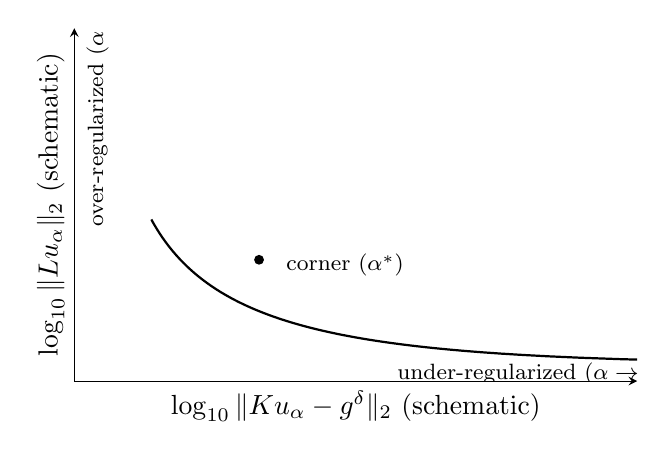
\begin{tikzpicture}
\begin{axis}[
 width=0.72\textwidth,
 height=0.5\textwidth,
 xlabel={$\log_{10}\|Ku_{\alpha}-g^{\delta}\|_2$ (schematic)},
 ylabel={$\log_{10}\|Lu_{\alpha}\|_2$ (schematic)},
 domain=0.05:6,
 samples=200,
 axis lines=left,
 every axis plot/.append style={thick, black},
 ticks=none,
 xmin=0, xmax=3.2,
 ymin=0, ymax=3.2,
]
\addplot[black, thick] ({0.15+ln(1+2/x)}, {0.15+ln(1+x/2.2)});
\node[draw, circle, fill=black, inner sep=1.1pt] at (axis cs:1.05,1.10) {};
\node[anchor=west] at (axis cs:1.15,1.05) {\footnotesize corner ($\alpha^{\ast}$)};
\node[anchor=north] at (axis cs:2.6,0.25) {\footnotesize under-regularized ($\alpha\to0$)};
\node[anchor=south, rotate=90] at (axis cs:0.25,2.6) {\footnotesize over-regularized ($\alpha\to\infty$)};
\end{axis}
\end{tikzpicture}
\caption{Schematic, illustrative L-curve generated from an explicit analytic filter-factor model (not measured or simulated diagnostic data), showing the corner separating the noise-amplification branch (small $\alpha$) from the over-smoothing branch (large $\alpha$). The point of maximum curvature, marked, is the L-curve estimate of $\alpha^{\ast}$.}
\label{ch14-fig:lcurve}
\end{figure}

Optimal-parameter-selection studies for Tikhonov-regularized EXAFS inversion benchmark the L-curve criterion against the discrepancy principle and GCV for an operator of comparable conditioning to the RFEA and Abel-inversion kernels here, finding the L-curve corner robust when the noise level is only approximately known -- the typical situation for laboratory sheath diagnostics \cite{ref0695}.

\section{Bayesian Formulation}
\label{sec:bayesian}

\subsection{Likelihood, Prior, and Posterior}

The deterministic regularization framework of \cref{sec:regularization} has an exact probabilistic counterpart that both justifies and generalizes it. The unknown $u$ is a random variable with a prior density $p(u)$ encoding everything believed, before any data are examined, about plausible sheath potentials, IEDFs, or density profiles -- smoothness, positivity, or bounds such as $f_{\mathrm{i}}(v) \ge 0$. The noisy data relate to $u$ through a likelihood $p(g^{\delta}\,|\,u)$ built from $\mathcal{F}$ and a noise model; for additive Gaussian noise with covariance $C_{\eta}$,
\begin{equation}
p(g^{\delta}\,|\,u) \propto \exp\!\left[ -\tfrac{1}{2} \left( g^{\delta} - \mathcal{F}[u] \right)^{\mathrm{T}} C_{\eta}^{-1} \left( g^{\delta} - \mathcal{F}[u] \right) \right].
\label{ch14-eq:likelihood}
\end{equation}
Bayes' theorem combines prior and likelihood into the posterior density,
\begin{equation}
p(u\,|\,g^{\delta}) = \frac{ p(g^{\delta}\,|\,u)\, p(u) }{ \int p(g^{\delta}\,|\,u')\, p(u')\, \mathrm{d}u' },
\label{eq:bayes}
\end{equation}
representing the complete state of knowledge about $u$ after the measurement. All subsequent inferences -- point estimates, error bars, and derived quantities such as $\Gamma_{E} = \int \tfrac{1}{2} m_{\mathrm{i}} v^{2} \cdot v f_{\mathrm{i}}(v)\, \mathrm{d}v$ -- are obtained by summarizing this posterior.

\subsection{Maximum A Posteriori Estimation and its Equivalence to Tikhonov Regularization}

The MAP estimator maximizes \cref{eq:bayes}, equivalently minimizing its negative logarithm. For a Gaussian prior $p(u) \propto \exp[-\tfrac{1}{2}(u-u_0)^{\mathrm{T}} C_{u}^{-1} (u-u_0)]$ with covariance $C_u$ and the Gaussian likelihood linearized as $\mathcal{F}[u] \approx Ku$,
\begin{equation}
u_{\mathrm{MAP}} = \arg\min_{u} \left\{ \left( g^{\delta} - Ku \right)^{\mathrm{T}} C_{\eta}^{-1} \left( g^{\delta} - Ku \right) + u^{\mathrm{T}} C_{u}^{-1} u \right\},
\label{eq:map}
\end{equation}
which, writing $C_{\eta} = \sigma_{\eta}^{2} I$ and $C_{u}^{-1} = (\alpha^2/\sigma_\eta^2) L^{\mathrm{T}}L$, is algebraically identical to \cref{ch14-eq:tikhonov}. This is a structural fact, not a coincidence: Tikhonov regularization \emph{is} Gaussian MAP estimation, and the choice of $L$ \emph{is} the choice of prior covariance $C_u$. TV regularization corresponds to a non-Gaussian (Laplace-type, heavy-tailed) prior on $u$'s derivative, which is why it tolerates occasional large jumps at a much lower probabilistic "cost" than a Gaussian prior would.

\subsection{Posterior Uncertainty and Credible Intervals}

Beyond the point estimate $u_{\mathrm{MAP}}$, the linear-Gaussian case yields the posterior covariance in closed form,
\begin{equation}
C_{\mathrm{post}} = \left( K^{\mathrm{T}} C_{\eta}^{-1} K + C_{u}^{-1} \right)^{-1},
\label{ch14-eq:posterior-cov}
\end{equation}
whose diagonal gives pointwise posterior variances -- and hence credible intervals -- for every component of $u$, including $\Gamma_{E}$ once propagated through the nonlinear moment integral, a substantive advantage over \cref{sec:regularization}, which supplies a single reconstruction $u_{\alpha}$ but no principled measure of confidence. The off-diagonal structure of $C_{\mathrm{post}}$ additionally reveals \emph{correlations} between reconstructed values at nearby velocities or radii, essential for propagating uncertainty into any derived quantity, since naively summing independent pointwise variances underestimates the true uncertainty.

Gaussian-process priors generalize the Gaussian $C_u$ above by specifying the prior covariance directly as a smooth kernel over the domain of $u$, rather than through a differential operator $L$. Bayesian modelling of Thomson-scattering and interferometer data with such priors demonstrates this in a magnetically confined plasma, jointly inferring density and temperature profiles with calibrated uncertainty bands and propagating them into derived quantities, directly analogous to propagating IEDF uncertainty into $\Gamma_{E}$ \cite{ref0683}. Bayesian inference from collective Thomson scattering on a transient gas-puff pinch extends the methodology to a rapidly evolving plasma, updating the posterior self-consistently as channels with different forward operators are combined \cite{ref0684}. A multi-instrument analysis system for divertor plasma characteristics fuses diagnostics -- each with its own $\mathcal{F}_j$ and likelihood $p_j(g_j^{\delta}\,|\,u)$ -- into a joint posterior $p(u\,|\,\{g_j^{\delta}\}) \propto p(u) \prod_j p_j(g_j^{\delta}\,|\,u)$, relevant whenever an energy flux estimate is cross-validated using RFEA, Langmuir-probe, and spectroscopic data \cite{ref0685}.

\subsection{Computational Considerations}

For nonlinear forward operators -- joint chord-integrated/collisional-radiative inversion, or nonlinear sheath-potential reconstruction -- the posterior of \cref{eq:bayes} is generally not Gaussian and \cref{ch14-eq:posterior-cov} does not apply exactly. It is then characterized either by local linearization about the MAP point (a Laplace approximation, \cref{ch14-eq:posterior-cov} with $K \to J[u_{\mathrm{MAP}}]$) or by direct Markov-chain Monte Carlo sampling, the price of a faithful characterization whenever nonlinearity or a non-Gaussian prior makes the Gaussian approximation inadequate.

\section{Plasma Tomography and Spectroscopic Inversion as Precedents}
\label{sec:tomography}

The ion-energy-flux inverse problems motivating this chapter belong to a larger family: recovering a spatially or spectrally resolved plasma quantity from indirect measurements. This section surveys that family for forward-operator structure, conditioning, and regularization strategies that transfer directly to sheath diagnostics.

\subsection{Geometric (Tomographic) Inversion}

Plasma tomography reconstructs a two- or three-dimensional emissivity, density, or temperature field from line-integrated (chord) measurements collected by cameras, bolometer arrays, or interferometers viewing the plasma from several directions. The forward operator is the Radon transform, or the Abel transform for axisymmetric sources viewed along one direction,
\begin{equation}
g(p, \theta) = \int_{-\infty}^{\infty} u(p\cos\theta - s\sin\theta,\ p\sin\theta + s\cos\theta)\, \mathrm{d}s,
\label{eq:radon}
\end{equation}
discretized into a sparse matrix $K$ whose rows are chords and columns are pixels or annular shells. The sparsity and limited-angle coverage of realistic chord geometries -- far fewer viewing directions than in medical or industrial tomography -- exacerbate the rank deficiency of \cref{sec:hadamard}, addressed by dedicated optical-tomography inversion algorithms that established the discretization, regularization, and error-propagation framework used throughout this literature. The Abel transform retains an analytic inversion formula in the noise-free limit, but a weak singularity near the symmetry axis makes the noisy inversion numerically delicate; treatments of Abel inversion for laser-induced plasma imaging address noise and incomplete data within a framework analogous to \cref{ch14-eq:tikhonov}.

\subsection{Spectroscopic Inversion}

A second precedent class arises when the forward operator involves a physically nonlinear spectroscopic model, typically a collisional-radiative model relating emissivity to $n_{\mathrm{e}}$ and $T_{\mathrm{e}}$. Radially resolved optical emission spectral imaging of atmospheric-pressure plasmas illustrates the combined geometric-and-spectroscopic problem, where the chord geometry and atomic model must be inverted jointly, not sequentially, to avoid propagating a geometric artifact into the spectroscopic interpretation -- relevant to sheath-adjacent OES or LIF signals unfolded both along the line of sight and through a nonlinear intensity-to-$f_{\mathrm{i}}(v)$ or $(n_{\mathrm{e}}, T_{\mathrm{e}})$ relationship.

A further relevant problem is recovering the electron energy distribution function from an indirect spectral signature. Regularized inversion of Bremsstrahlung emission spectra from pulse-height data shows that count-based (Poisson) noise models -- appropriate whenever data are photon or particle counts, as for energetic-particle diagnostics near a sheath -- require a modified likelihood and regularization functional matching low-count-rate statistics rather than the Gaussian Tikhonov framework.

\subsection{Transfer to Sheath and Ion-Energy-Flux Diagnostics}

The unifying lesson is that the pathology afflicting sheath-adjacent inverse problems -- RFEA differentiation, Abel-type inversion of chord-integrated OES or LIF signals, joint geometric-spectroscopic unfolding of $(n_{\mathrm{e}}, T_{\mathrm{e}})$ feeding into $u_{\mathrm{B}}$ and hence $\Gamma_{E}$ -- is not a peculiarity of sheath physics but an instance of a well-characterized problem class. Every tool surveyed in \cref{sec:regularization,sec:bayesian} transfers with no change in mathematical structure, only in the form of $\kappa(x,x')$ and the choice of $L$ or $C_u$.

\section{Conditioning, Resolution, and Error Propagation}
\label{sec:conditioning}

\subsection{Condition Number}

The numerical severity of an inverse problem's ill-posedness is summarized by
\begin{equation}
\kappa(K) = \frac{\sigma_{\max}}{\sigma_{\min}},
\label{eq:condition-number}
\end{equation}
with $\sigma_{\max}, \sigma_{\min}$ the largest and smallest nonzero singular values of $K$. A large $\kappa(K)$ signals a poorly constrained solution space; for RFEA, Abel, and collisional-radiative kernels, $\kappa(K)$ at any practical discretization is typically many orders of magnitude, confirming \cref{sec:hadamard}. Regularization replaces $K$ by $K_{\alpha}^{\dagger}$, whose effective condition number on the recovered subspace is finite.

\subsection{Resolution and the Averaging Kernel}

A regularized reconstruction does not recover the true $u$ exactly even without noise, since the filter factors of \cref{eq:tikhonov-svd} (or the truncation of \cref{eq:tsvd}) suppress high-index components regardless of whether they carry noise or signal. This systematic distortion is characterized by the \emph{resolution} or \emph{averaging-kernel} matrix,
\begin{equation}
R_{\alpha} = K_{\alpha}^{\dagger} K, \qquad u_{\alpha} = R_{\alpha}\, u_{\mathrm{true}} + \left(\text{noise term}\right),
\label{eq:resolution-matrix}
\end{equation}
which reduces to the identity in the unregularized limit and otherwise smears $u_{\mathrm{true}}$: the $i$-th row of $R_\alpha$ describes which combination, and over what width, of $u_{\mathrm{true}}$ contributes to $u_{\alpha,i}$. Its full width at half maximum is the rigorous definition of resolution -- sharper means finer resolution but, through \cref{eq:tikhonov-svd}, smaller $\alpha$ and larger noise amplification via \cref{eq:noise-amplification}. No choice of $\alpha$ escapes this trade-off; every reported reconstruction in this monograph implicitly states a chosen point on this curve, not the "true," fully resolved quantity.

\subsection{Error Propagation into Derived Quantities}

The physical target of this monograph is a nonlinear functional of the reconstructed IEDF,
\begin{equation}
\Gamma_{E} = \int_{0}^{\infty} \tfrac{1}{2} m_{\mathrm{i}} v^{2} \cdot v\, f_{\mathrm{i}}(v)\, \mathrm{d}v,
\label{eq:energy-flux-functional}
\end{equation}
so the uncertainty in $\Gamma_{E}$ must be obtained by propagating the full posterior (or regularized) covariance of $f_{\mathrm{i}}(v)$ through this integral, not by averaging pointwise uncertainties. To first order, with sensitivity kernel $w(v) = \tfrac{1}{2}m_{\mathrm{i}}v^{3}$,
\begin{equation}
\mathrm{Var}[\Gamma_{E}] \approx \iint w(v)\, C_{\mathrm{post}}(v,v')\, w(v')\, \mathrm{d}v\, \mathrm{d}v',
\label{ch14-eq:error-propagation}
\end{equation}
depending on the full off-diagonal structure of $C_{\mathrm{post}}(v,v')$. Because $w(v) \propto v^3$ emphasizes the high-velocity tail of $f_{\mathrm{i}}(v)$ -- precisely where the RFEA differentiation problem is least well resolved, since high energies sample the sparse extreme of the sweep -- the propagated uncertainty on $\Gamma_{E}$ is dominated by the poorly resolved tail, not the well-resolved bulk. Reporting a point estimate without correctly propagated, correlation-aware uncertainty is a common and consequential error.

\subsection{Diagnosing Resolution Loss in Practice}

$R_{\alpha}$ and $C_{\mathrm{post}}$ are both computable at $\alpha^{\ast}$ directly from the SVD or Cholesky factorization already required for the reconstruction, so reporting resolution and correlated uncertainty costs little extra. The L-curve corner, filter factors, resolution matrix, and propagated uncertainty together form a diagnostic package that should accompany any reconstructed sheath quantity: a point estimate alone is not scientifically complete given \cref{sec:hadamard}.

\section{Summary}

This chapter treats the recovery of sheath and plasma quantities from indirect diagnostic data as a genuine inverse problem. The forward operator $\mathcal{F}$ -- whether the transform relating an RFEA sweep to $f_{\mathrm{i}}(v)$, a chord-integrating geometric integral, or the nonlinear map of a collisional-radiative model -- is generically smoothing, and its inversion is ill-posed in the sense of Hadamard: existence is restored by a least-squares formulation, while uniqueness and stability remain compromised by a near-null space and singular-value decay that amplifies noise without bound in the naive pseudoinverse. Regularization -- Tikhonov, truncated SVD, and total variation -- restores a controlled, stable dependence on the data by penalizing noise-dominated components, at an unavoidable cost in resolution captured by the averaging-kernel matrix; the trade-off is set by the L-curve criterion or related discrepancy-based and cross-validation rules. The Bayesian formulation subsumes this picture, identifying MAP estimation under a Gaussian prior with Tikhonov regularization while furnishing a full posterior from which credible intervals and correlations follow directly, and extending to non-Gaussian priors, nonlinear operators, and multi-diagnostic fusion. Plasma tomography and spectroscopic inversion provide validated precedents that transfer directly to sheath and ion-energy-flux diagnostics: the same pathologies, remedies, and resolution-versus-noise trade-off govern both. Its central conclusion is that any reconstructed sheath quantity -- an IEDF, a potential profile, a density or temperature profile, or $\Gamma_{E}$ itself -- is scientifically incomplete without a correctly propagated statement of its resolution and correlated uncertainty, tools that are a low-cost byproduct of the regularized or Bayesian inversion procedure by which the quantity was obtained.
